 

\actTitle{Worksheet 1.1}

\videoLink{Section 1.1}{https://www.youtube.com/playlist?list=PLYHZK3b8UFw3ad1wlhTMGcL5kgita6QGS}

\noindent
Student goals:
  \begin{itemize}
  \item Plot points in the coordinate plane.
  \item Identify the four quandrants of the coordinate plane.
  \item Calculate the distance between two points.
  \item Make rough sketch of the graph of a function by plotting
    points first.
  \item Determine the $x$ and $y$ intercepts of a function
    analytically and graphically.
  \end{itemize}


\noindent \textbf{Instructions:}  Work together in groups of  3 or 4 to complete the following problems.


\begin{enumerate}

\item Mark the points $P_1(-2,-4.5)$ and $P_2(4,1.5)$ on the
  coordinate plane below. Determine the distance between the two
  points.  Include a sketch of a right triangle whose hypotenuse
  represents the distance between the two points. Label the lengths of
  each side of the right triangle.

  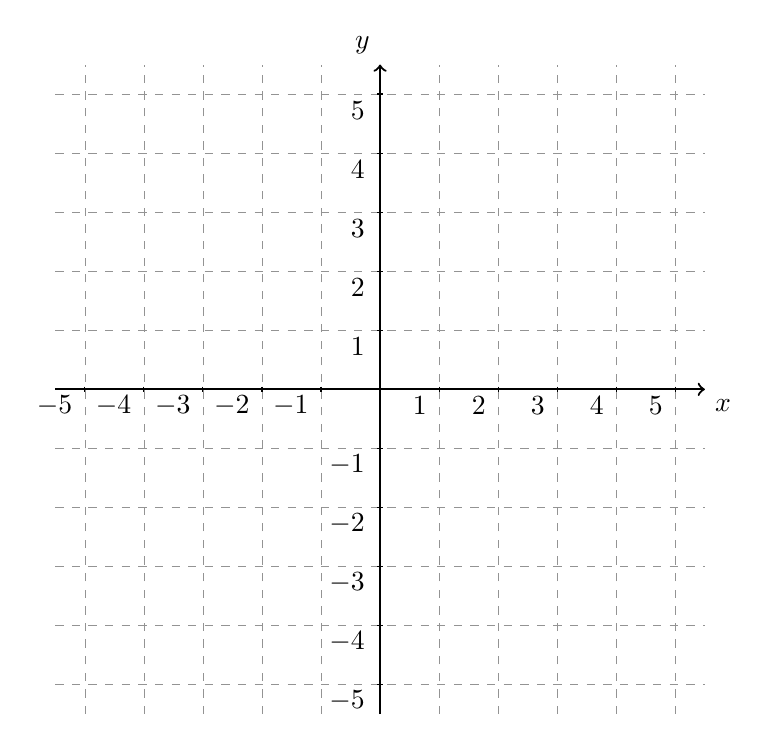
\begin{tikzpicture}[y=0.75cm, x=0.75cm,font=\sffamily]
    % bounds
    % ticks
    \draw[step = 1, gray, very thin,dashed,opacity=0.85] (-5.5, -5.5) grid ( 5.5,5.5);
 	% axis
	\draw[thick,->] (-5.5,0) -- coordinate (x axis mid) (5.5,0) node[anchor = north west] {$x$};
    \draw[thick,->] (0,-5.5) -- coordinate (y axis mid) (0,5.5) node[anchor = south east] {$y$};
    \foreach \y in {-5,-4,...,-1,1,2,...,5.5} {
      \draw (1pt, \y) -- (-1pt, \y) node[yshift=-6,xshift=-1,anchor=east] {$\y$};
    }
    \foreach \x in {-5,-4,...,-1,1,2,...,5.5} {
      \draw (\x,1pt) -- (\x,-1pt) node[yshift=-5,xshift=-1,anchor=east] {$\x$};
    }
  \end{tikzpicture}


\newpage


\item Find the $x$ and $y$ intercepts of the following equations.
\begin{enumerate}
\item $x^2+y=9$
\vfill
\item $y=|x+4|-3$
\end{enumerate}
%\item Determine the distance between the points $A(-3, 4)$ and  $C(4, -8)$. \\[2.5in]
\vfill

\newpage

\item Determine all points lying on the $y$-axis that are 5 units away
  from the point $(4,-2)$.  Use the problem solving process stated
  below, and explicitly identify which part of the process you are
  using in each of your steps.  As a group, write your complete
  solution on the board.


\begin{boxthm}
{\bf Problem Solving Process}
\begin{enumerate}
\item Re-read the problem.
\item Determine what the problem is asking for along with the format of that answer.
\item Circle/Underline the important components of the problem.
\item Determine the topics/concepts being assessed.
\item Write down relevant formulas, definitions, and equations.
\item Discuss your ideas with your group.
\item Solve the problem and verify that your solution answers the question in the correct format.
\end{enumerate}

\end{boxthm}
\vfill
\newpage

\item Use the following parts to find all points on the line $y=2x$ that are 5 units away from $P(-1,3)$.  
\begin{enumerate}
\item Find the points $(x,y)$ on the line $y=2x$ for $x=1, -2,$ and $5$.
\vfill
\item What if we didn't know the value of $x$?  Write an ordered pair formula that works for every point on the line $y=2x$?\vfill
\item Use part (b) to find all points on the line $y=2x$ that are 5 units away from $P(-1,3)$. 
\vfill
\vfill
\vfill
\end{enumerate}
\newpage





\end{enumerate}




\hwTitle{Homework Section 1.1}

\begin{enumerate}
\item The points $ABC$ form a triangle.
  \begin{enumerate}
  \item Plot $A(-1,2),B(3,0) , C(4,2), $ and draw the triangle on the graph below.\\

    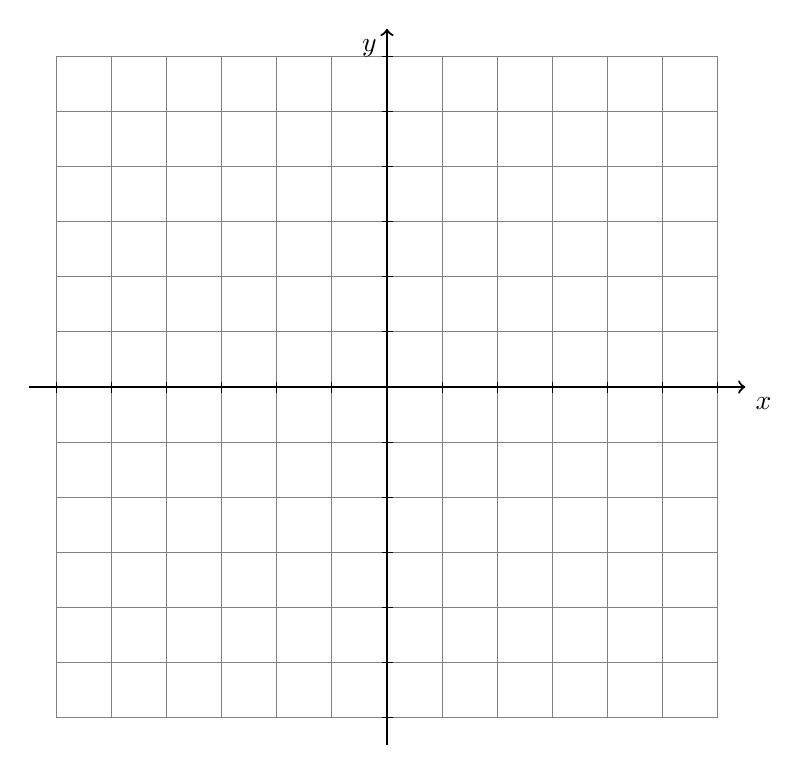
\begin{tikzpicture}[y=.7cm, x=.7cm,font=\sffamily]
      %% ticks
      \draw[step = 1, gray] (-6,-6) grid (6,6);
      %% axis
      \draw[thick,->] (-6.5,0) -- coordinate (x axis mid) (6.5,0) node[anchor = north west] {$x$};
      \draw[thick,->] (0,-6.5) -- coordinate (y axis mid) (0,6.5) node[anchor = north east] {$y$};
      \foreach \y in {-6,-5,...,-1,1,2,...,6} {
        \draw (2pt, \y) -- (-2pt, \y);
      }
      \foreach \x in {-6,-5,...,-1,1,2,...,6} {
        \draw (\x,2pt) -- (\x,-2pt);
      }

    \end{tikzpicture}

  \item Determine the perimeter of the triangle.
  \item Is the triangle a right triangle?  Show work to support your answer.
  \end{enumerate}
  
\end{enumerate}
